\documentclass[12pt,oneside]{book}
\pagestyle{headings}

% Note that the line below could be modified to suit a
% particular system since the "geometry" package behaves
% differently in Unix, Windows and Mac, especially for the
% top margins.
% Adjust the parameter "top" (measuring the height of the
% space allocated to a header) and "headsep" (measuring
% the distance from the bottom of the header to the
% first line of text.
\usepackage[top=1.3in,left=1.5in,bottom=1in,right=1in,headsep=0.5in]{geometry}

\usepackage{setspace}
\onehalfspacing
%\doublespacing

% Headers and footers for thesis
\usepackage{fancyhdr}

\markboth{}{}
\newcommand\startchapter[1]{\chapter{#1}\thispagestyle{myheadings}}
\newcommand\startappendix[1]{\chapter{#1}\thispagestyle{myheadings}}
\newcommand\startfirstchapter[1]{\chapter{#1}}

% Manual addition of section to Table of Contents
\newcommand\TOCadd[1]{\newpage\phantomsection\addcontentsline{toc}{chapter}{#1}}

% Float Customization
\renewcommand{\floatpagefraction}{0.01}

% Customization of Tables of Contents and List of Figures/Tables
\usepackage{tocloft}
\renewcommand\cfttabpresnum{Table\ }
\renewcommand\cfttabnumwidth{0.75in}
\renewcommand\cftfigpresnum{Figure\ }
\renewcommand\cftfignumwidth{0.80in}
\newcommand{\HRule}{\rule{\linewidth}{0.5mm}}
% Long Table and decimal aligned columns
\usepackage{dcolumn}
\usepackage{longtable}

% Mathematics support
\usepackage{amsmath}
\usepackage{amsthm}
\usepackage{amssymb}


% Text Control
\usepackage{xspace}
\usepackage{textcase}

% Graphics
\usepackage{wasysym}
\usepackage{graphics}
\usepackage{graphicx}   % A package to allow insertion of
                        % external image files

% rohith specific packages
\usepackage[hidelinks]{hyperref}
\usepackage{xcolor}
\usepackage{textcomp}
\usepackage{listings}
\usepackage[listings, many]{tcolorbox}
\usepackage[OT1]{fontenc} 
\usepackage{color}
\usepackage{hyperxmp}


% colors
\definecolor{lightgray}{rgb}{.9,.9,.9}
\definecolor{codegreen}{rgb}{0,0.6,0}
\definecolor{codegray}{rgb}{0.5,0.5,0.5}
\definecolor{codepurple}{rgb}{0.58,0,0.82}
\definecolor{backcolour}{rgb}{0.95,0.95,0.92}

\lstdefinelanguage{JavaScript}{
  keywords={typeof, new, true, false, catch, function, return, null, catch, switch, var, if, in, while, do, else, case, break, console, const},
  keywordstyle=\color{blue},
  ndkeywords={class, export, boolean, throw, implements, import, this, for},
  ndkeywordstyle=\color{magenta},
  identifierstyle=\color{black},
  sensitive=false,
  comment=[l]{//},
  morecomment=[s]{/*}{*/},
  commentstyle=\color{codegreen}\ttfamily,
  stringstyle=\color{red}\ttfamily,
  morestring=[b]',
  morestring=[b]"
}

\lstset{
  language=JavaScript,
  backgroundcolor=\color{lightgray},
  extendedchars=true,
  basicstyle=\footnotesize\ttfamily,
  showstringspaces=false,
  showspaces=false,
  numberstyle=\footnotesize,
  numbersep=9pt,
  tabsize=2,
  breaklines=true,
  showtabs=false,
  captionpos=b
}

\lstdefinestyle{mystyle}{
    backgroundcolor=\color{backcolour},   
    commentstyle=\color{codegreen},
    keywordstyle=\color{magenta},
    numberstyle=\tiny\color{codegray},
    stringstyle=\color{codepurple},
    basicstyle=\ttfamily,
    breakatwhitespace=false,         
    breaklines=true,                 
    captionpos=b,                    
    keepspaces=true,                 
    numbers=left,                    
    numbersep=5pt,                  
    showspaces=false,                
    showstringspaces=false,
    showtabs=false,                  
    tabsize=2
}
\lstset{style=mystyle}
\lstset{escapeinside={\%*}{*)}}


%% rohith commands
\newcommand{\AIDE}{AI-supported programming}%{AI-driven development}
\newcommand{\AISE}{AI-supported software development}%{AI-driven software engineering}
\newcommand{\cct}{AI-supported code completion tools}
\newcommand{\repl}{replication package at \url{todo}}

%% table wrap text helper
\newcolumntype{L}{>{\centering\arraybackslash}m{.42\linewidth}}

\begin{document}

% Front Matter
\input frontmatter/fm

\newpage

	\startfirstchapter{Introduction}
\label{chapter:introduction}
Programming is a powerful and ubiquitous problem-solving tool. Developing systems that can assist software developers or even generate programs independently could make programming more productive and accessible. 
Code completion is a feature that predicts what a software developer is trying to code and offers predictions as suggestions to the user. All modern IDEs feature intelligent code completion tools in different forms and it is used by both new and experienced software developers. Developing AI systems that can effectively model and understand code can transform these code completion tools and the way we interact with them.

Recent large-scale pre-trained language models such as \cop{}~\cite{Copilot-web} have demonstrated an impressive ability to generate code and are now able to solve programming contest style problems~\cite{empirical_eval}. 
However, software engineering is much more than writing code, it involves complex challenges like choosing the best practices, avoiding code smells, using design patterns and many more decisions before writing code. 
The scope of capabilities for \cct{} is uncertain. Identifying the nature of \cop{} capabilities when it comes to more complex challenges, i.e., \AISE{} (as opposed to development tasks, such as coding or programming problems). Delineating where \cct{} are currently best able to perform, and where more complex software engineering tasks overwhelm them is helpful in answering questions like 
Exactly which software problems can current \cct{} solve? 
If \cct{} makes a suggestion, is that suggestion accurate and optimal? Should a user intervene to correct it? But identifying these boundaries is a challenging task. In the next section, we discuss this challenge and the research opportunity that it creates as the motivation for this study.

\section{Motivation}


In this thesis, we investigate the

\section{\cct{}}




\section{Problem Statement and Research Questions}
The overarching goal of this study is to:
\begin{quote}
    Identify the boundaries of the capabilities of GitHub Copilot. Toward this goal, we compare Copilot code suggestions against well known language idioms and code smells. Additionally, we introduce a simple taxonomy of software abstraction hierarchies to show different capability levels of \cct{}. 
\end{quote}

The capabilities and the limitations of current \cct{} like Copilot are unknown, identifying the limitations of \cct{} would help the users use the tool effectively and focus more on the tasks \cct{} are shown to be not useful. 
The objective of this study is to achieve a better understanding of the areas Copilot performs better than a human and the areas where Copilot performs worse than a human. We conduct an exploratory study with the following research objectives:

\begin{enumerate}
  \item[\textbf{RQ-1: }]
  \textbf{What are the current boundaries of \cct{}?} \\
  \textbf{Approach -} We use GitHub's Copilot as a representative for \cct{}. We explore Copilot's code suggestions for code smells and usage of language idioms. We conduct additional investigation to determine the current boundaries of Copilot by introducing a taxonomy of software abstraction hierarchies where ‘basic programming functionality’ such as code compilation and syntax checking is at the least abstract level. Software architecture analysis and design is at the most abstract level. 
  
  \item[\textbf{RQ-1.1: }]
  \textbf{How do \cct{} manage programming Idioms?} \\
  \textbf{Approach -} We examine Copilot code suggestions on top 25 idioms used in open source projects sampled from work of Alexandru et al.~\cite{Alexandru2018}, which identified idioms from presentations given by renowned Python developers. We investigate how Copilot's top code suggestion compares to Python idioms from Alexandru et al.~\cite{Alexandru2018}. In addition, we report if the idiom is listed in any of the 10 viewable suggestions from Copilot.
  
  \item[\textbf{RQ-1.2: }]
  \textbf{How do \cct{} manage manage to suggest non-smelly code?} \\
\textbf{Approach -} We examine Copilot code suggestions on 25 different best practices sampled from AirBNB JavaScript coding style guide~\cite{airbnb_code}. We investigate how Copilot's top code suggestion compares to the best practices in AirBNB JavaScript coding style guide~\cite{airbnb_code}. Additionally, we report if the best practice is listed in any of the 10 viewable suggestions from Copilot. 
 
  \item[\textbf{RQ-2: }]
  \textbf{Given the current boundary, how far is it from suggesting design decisions which seem much beyond the boundary??} \\
  \textbf{Approach -} Based on our findings in RQ-1, we discuss how far current \cct{} are from the design level in our taxonomy. We look at current limitations of Copilot and provide recommendations on how to make current \cct{} reach design abstraction level. Additionally, we report on ethical considerations, explainability and control of \cct{} like Copilot. 
\end{enumerate}
\section{Contributions}
\section{Thesis Outline}



	\startchapter{Background \& Related Work}
\label{chapter:background}

\newlength{\savedunitlength}
\setlength{\unitlength}{2em}

\section{Introduction}

\section{\cct{} Journey}

\subsection{Before Copilot}

\subsection{Alternatives to Copilot}
\section{\cct{} related works}
\section{Challenges with \cct{}}
\label{challenges}
Some of these basic programming challenges have been already documented and are, we suspect, very much under consideration by the corporate teams behind Copilot and Codex. Since these tools are trained on existing software source code, and training costs are expensive, several classes of errors have been discovered, which follow from the presence of these same errors in public (training) data.

Copilot can make simple coding mistakes, such as not allowing for an empty array in a sort routine\footnote{all examples are documented in our \repl{}.}. Copilot does not understand security vulnerabilities, so it will suggest code that allows for a \textsf{log4shell} vulnerability\footnote{\url{https://www.wiz.io/blog/10-days-later-enterprises-halfway-through-patching-log4shell/}}, or common SQL injection attacks. A recent study by Pearce et al.~\cite{copilot_security} showed that approximately 40\% of the code suggested by Copilot is found to be vulnerable, when tested on 89 different scenarios for Copilot to complete.
Similarly, concerns have been raised about Copilot licence compliance and copyright violation~\cite{code_clone}; with similar input data, Copilot suggests identical code to existing code on GitHub, which may be under copyright. 

% Karampatsis et al.~\cite{github_bugs} showed that for the 1000 most popular open-source Java repositories on GitHub, there is a frequency of one single statement bug per 1600-2500 lines of code and about 33\% of all the bugs match a set of 16 bug templates. This shows that there are bugs which occur repeatedly in the public repositories of GitHub, which can make Copilot biased to suggest bug prone code over bug-free versions.
As it is trained on public data collected in May 2020 from 50 million public repositories on GitHub~\cite{copilot}, any code uploaded after that date is absent in the knowledge base of Copilot. 
% The training data for Copilot was collected in May 2020 from 50 million public repositories on GitHub~\cite{copilot}. 
%It does not have any data uploaded to GitHub after that date and any data from useful sources like documentation and Stack Overflow to improve its suggestions from commonly occurring bugs.
Any software flaws present in large numbers on GitHub will tend to dominate the learning of the model.

But these challenges are not surprising, and have straightforward fixes.
Fixes might include better data engineering and filtering, to remove known problems. This is already part of the training of these large language models, although the exact process has not been publicly disclosed. 
Similarly, it seems viable to conduct security scans or linting runs prior to making a suggestion, in order to remove obvious problems like SQL injection. 
Clone detection techniques can help find places where code violates copyright. 
Better machine learning approaches, using active learning or fine-tuning, might help learn local lessons~\cite{Menzies2013} for customization in the case of identifier naming or formatting.
In most of these cases, good tools exist already for this. 

Our belief is that while heuristic, such flaws can be fixed and will be fixed in short order. 
What we believe is harder to fix will be problems where straight-forward corrections may not exist and rules for finding problems are harder to specify than those in smell detectors or linters ~\cite{Ernst2017}.

\section{Chapter Summary}
In this chapter, we first provided some background on different language models used for \cct{} and their limitations. We reviewed early developments in \cct{} with statistical language models like N-grams. Followed by a discussion on N-gram based \cct{} and the limitations of statistical language models, resulting in using neural language models for \cct{}. We established the importance of transformers for \cct{} which is a crucial component of OpenAI's Codex Model~\cite{copilot}. To further explore the role of transformer architecture in \cct{}, we reviewed studies showing context-sensitive contextualised word representations were presented by LMs such BERT~\cite{bert}.

We then discussed GitHub Copilot, the \cct{} we would use as the basis for our study in this thesis. Additionally, we reviewed the key functionalities of Copilot.
Furthermore, we discussed some of the related works on Copilot about its usage~\cite{Vaithilingam2022} and its effectiveness in solving programming contest style problems~\cite{empirical_eval}. We concluded by introducing some of the other \cct{} that provide similar functionality like Copilot.

In the next chapters, we discuss the problems with using \cct{} like Copilot that are harder to fix and straight-forward corrections may not exist, like language idioms and code smells. 
We try to address \textbf{RQ-1} (What are the current boundaries of code completion tools) using the methodology and present our results~(Chapter~\ref{chapter:methodology}).
We then introduce a taxonomy of software abstraction hierarchy to help with finding the current boundaries of \cct{} like Copilot (Chapter~\ref{chapter:framework}). We address \textbf{RQ-2} (Given the current boundary, how far is it from suggesting design decisions?) with a discussion of the complex nature of design decisions, and the challenges with trying to use \cct{} to make design decisions.
Finally, we discuss some of the practical implications, limitations of our findings and also provide some future directions to help further research in \cct{} (Chapter~\ref{chapter:discussion}).

\setlength{\unitlength}{\savedunitlength}

	\startchapter{Challenges with Copilot}
\label{chapter:methodology}

\section{Introduction}
Useful \cct{} should always suggest recommended coding best practices in its first suggestion. In this chapter, we test if Copilot suggests the recommended ways sampled from popular sources.
We begin by explaining the current challenges with \cct{} like Copilot, showing recent research works on common problems faced with using Copilot and the motivation to find the limitations of current \cct{} like Copilot~(section~\ref{challenges}).

In section~\ref{methodology}, we explain our approach to \textbf{RQ-1} (What are the current boundaries of \cct{}?). 
We describe our sampling approach to collecting Pythonic idioms~(section~\ref{sampling}) and best practices in JavaScript~(section~\ref{smells:sampling}). We then describe the input given to Copilot for triggering the generation of code suggestions~(section~\ref{input}).
Finally, we explain our evaluation method to compare Copilot suggestions to the recommended practices~(section~\ref{evaluation}).

In section~\ref{results}, we present our results on performance of Copilot in suggesting recommended practices for 50 different coding scenarios~(25 pythonic idioms + 25 code smells), which answers \textbf{RQ-1.1} (How do \cct{} manage programming idioms?), and \textbf{RQ-1.2} (How do \cct{} manage to write non-smelly code?).
We observe that Copilot had the recommended practices in its top 10 suggestions for 18 out of 50 coding scenarios~(36\% of all tests performed).

% In section~\ref{methodology}, we describe our sampling approach to collecting python idioms and the evaluation method used to compare Copilot suggestions to the optimal way listed in python idioms. In section~\ref{secidioms}, we show the results of the study comparing Copilot suggestions and idioms in python programming language. We observe that Copilot performs poorly in suggesting the optimal way in its suggestions. 

% Having identified the performance of current \cct{} like Copilot on detecting and suggesting common patterns like language idioms in chapter~\ref{chapter:idioms}, in this chapter we test if Copilot suggests code that follows code review standards.
% We begin by explaining our approach to \textbf{RQ-1.1} (How do \cct{} manage to write non-smelly code?). To achieve this, we conduct an exploratory study to find if \cct{} tools like Copilot suggest the best practices based on code review standards in their suggestions. 

% In section~\ref{smells:methodology}, we describe our sampling approach to collecting best practices in javascript and the evaluation method used to compare Copilot suggestions to the best practices listed in coding style and code review standards. 
% In section~\ref{bp}, we show the results of the study comparing Copilot suggestions and code review standards in javascript.

\section{Background \& Motivation}
\label{challenges}
Code completion tools are very useful but are often limited to the generation of single elements (e.g., method calls and properties) and the usage of templates. 
Furthermore, too many recommendations can decrease the usefulness of the tool~\cite{Proksch2015}. 
\cct{} must be accurate with its code suggestions while minimizing the number of different code suggestions recommended to the user.

Copilot can make simple coding mistakes, such as not allowing for an empty array in a sort routine\footnote{all examples are documented in our \repl{}.}. Copilot does not understand security vulnerabilities, so it will suggest code that allows for a \textsf{log4shell} vulnerability\footnote{\url{https://www.wiz.io/blog/10-days-later-enterprises-halfway-through-patching-log4shell/}}, or common SQL injection attacks. A recent study by Pearce et al.~\cite{copilot_security} showed that approximately 40\% of the code suggested by Copilot is vulnerable when tested on 89 different scenarios for Copilot to complete.
Some of these basic programming challenges have been already documented and are, we suspect, very much under consideration by the corporate teams behind Copilot and Codex. 
Since these tools are trained on existing software source code and training costs are expensive, several classes of errors have been discovered, which follow from the presence of these same errors in public (training) data.
Similarly, concerns have been raised about Copilot license compliance and copyright violation~\cite{code_clone}; with similar input data, Copilot suggests identical code to existing code on GitHub, which may be under copyright. 
As it is trained on public data collected in May 2020 from 50 million public repositories on GitHub~\cite{copilot}, any code uploaded after that date is absent in the knowledge base of Copilot. 
% The training data for Copilot was collected in May 2020 from 50 million public repositories on GitHub~\cite{copilot}. 
%It does not have any data uploaded to GitHub after that date and any data from useful sources like documentation and Stack Overflow to improve its suggestions from commonly occurring bugs.

Karampatsis et al.~\cite{github_bugs} showed that for the 1000 most popular open-source Java repositories on GitHub, there is a frequency of one single statement bug per 1600-2500 lines of code and about 33\% of all the bugs match a set of 16 bug templates. 
So, any software flaws present in large numbers on GitHub will tend to dominate the learning of the model.
But these challenges are not surprising and have straightforward fixes. These fixes might include better data engineering and filtering to remove known problems, like a filter introduced by GitHub to suppress code suggestions containing code that matches public code on GitHub, although the exact filtering process has not been publicly disclosed.

Similarly, it seems viable to conduct security scans or linting runs before suggesting removing obvious problems like SQL injection. 
Clone detection techniques can help find places where code violates the copyright. 
Better machine learning approaches, using active learning or fine-tuning, might help learn local lessons~\cite{Menzies2013} for customization in the case of identifier naming or formatting.
In most of these cases, good tools exist already for this. 

Although these are clearly challenges, Copilot seems already to be on its way to fixing them, like a filter introduced by GitHub to suppress code suggestions containing code that matches public code on GitHub. 
However, what is more difficult to envision are the problems that are harder to fix because straightforward corrections may not exist, and rules for finding problems are more challenging to specify than those in smell detectors or linters~\cite{Ernst2017} like language idioms and code smells.

Developers often discuss software architecture and actual source code implementations in online forums, chat rooms, mailing lists, or in person. 
Programming tasks can be solved in more than one way. 
The best way to proceed can be determined based on case-specific conditions, limits, and conventions. Strong standards and a shared vocabulary make communication easier while fostering a shared understanding of the issues and solutions related to software development.
However, this takes time and experience to learn and use idiomatic approaches~\cite{Alexandru2018}.

\cct{} can help steer users into using more idiomatic approaches with its code suggestions or vice-versa.
This makes it crucial to find the boundaries of \cct{} like Copilot~(\textbf{RQ 1}) and create a clear understanding of where can we use \cct{} like Copilot and where should the user be vigilant in using \cct{} code suggestions.
To achieve this, we conduct an exploratory study to find if \cct{} tools like Copilot suggest the recommended best coding practices in their suggestions.
\section{Methodology}
\label{methodology}
In this section, We explain the methodology we used to address \textbf{RQ-1} (What are the current boundaries of \cct{}?). We perform our experiments Copilot suggestions on Pythonic Idioms~(section~\ref{idioms}) and code smells in JavaScript~(section~\ref{smells}).

Additionally, we explain how 25 coding scenarios for Pythonic idioms~(section~\ref{smells:sampling}) and code smells in JavaScript~(section~\ref{sampling}) were sampled.
Finally, we discuss how the input is shaped to trigger Copilot to generate code suggestions~(section~\ref{input}) and how Copilot suggestions are evaluated (section~\ref{evaluation}).
The following analysis was carried out using the Copilot extension in Visual Studio Code. We use the most recent stable release of the Copilot extension available at the time of writing~(version number 1.31.6194) in Visual Studio Code.

\subsection{Pythonic Idioms}
\label{python}
A software language is more than just its syntax and semantics; it is also a set of known effective ways to address real-world issues using it. 
To answer \textbf{RQ-1.1} (How do \cct{} manage programming idioms?),
we chose Python, one of the most popular programming languages, because Copilot's base model Codex performs best in Python~\cite{copilot}.  

The definition for the term \emph{Pythonic} in Python found in official Python glossary\footnote{\url{https://docs.python.org/3/glossary.html\#term-pythonic}} as follows:

\begin{quote}
    An idea or piece of code follows the most common idioms of the Python language rather than implementing code using concepts common to other languages. For example, a common idiom in Python is to loop over all elements of an iterable using a for statement. Many other languages do not have this construct, so people unfamiliar with Python sometimes use a numerical counter instead, instead of the cleaner, pythonic method.
\end{quote}

This definition indicates a broad meaning, referring to both concrete code and also \emph{Ideas} in a general sense. Many Python developers argue that coding the \emph{pythonic way} is the most accepted way to code by the Python community~\cite{Alexandru2018}. 
We consider an \emph{idiom} to be any reusable abstraction that makes Python code more readable by shortening or adding syntactic sugar. Idioms can also be more efficient than a basic solution, and some idioms are more readable and efficient.
The pythonicity of a piece of code stipulates how concise, easily readable, and generally good the code is. This concept of pythonicity, as well as the concern about whether code is pythonic or not, is notably prevalent in the Python community.

We sampled idioms from the work of Alexandru et al.~\cite{Alexandru2018}, and Farook et al.~\cite{idioms}, which identified idioms from presentations given by renowned Python developers that frequently mention idioms, e.g., Hettinger~\cite{hettinger} and Jeff Knupp~\cite{knupp} and 
popular Python books, such as ``Pro Python''~\cite{Alchin2010}, ``Fluent Python''~\cite{fluent}, ``Expert Python Programming''~\cite{expert}.


\subsubsection{Sampling Approach}
\label{sampling}
We sampled the top 25 popular pythonic idioms found in open source projects based on the work of Alexandru et al.~\cite{Alexandru2018}, and Farook et al.~\cite{idioms}.
The decision to sample \emph{most popular} pythonic idioms is taken to give the best chance for Copilot to suggest the pythonic way as its top suggestion. As a result, Copilot will have the pythonic way more frequently in its training data and more likely to suggest the pythonic way in its suggestions.
However, Copilot is closed source, and we cannot determine if the frequency of code snippets in training data affects Copilot's suggestions. Research by GitHub shows that Copilot can sometimes recite from its training data in ``generic contexts"\footnote{\url{https://github.blog/2021-06-30-github-copilot-research-recitation/}}, which may lead to potential challenges like license infringements~(shown in section~\ref{challenges}). 
Sampling the most frequently used idioms will also help understand if Copilot can recite idioms present in its training data~(GitHub public repositories), which is the ideal behavior for \cct{}.

\subsection{Code Smells}
\label{smells}
A standard style guide is a set of guidelines that explain how code should be written, formatted and organized. 
Using a style guide ensures that code can be easily shared among developers. As a result, any new developer may immediately become familiar with a specific piece of code and write code that other developers will quickly and easily comprehend.
A good \cct{} tool should only suggest code consistent with coding style and pass code reviews by humans. 

To answer \textbf{RQ-1.2} (How do \cct{} manage to suggest non-smelly code?), we chose JavaScript to generalize our experiments with Copilot. 
We relied on the AirBNB javascript coding style guide~\cite{airbnb_code}, a widely used coding style and code review standard introduced in 2012, described as a ``primarily reasonable approach to JavaScript''~\cite{airbnb_code}.

% \section{Methodology}
% \label{smells:methodology}
% In this Section, we explain the methodology we used to address \textbf{RQ-1.2} (How do \cct{} manage to suggest non-smelly code?), including how the best practices were sampled (section~\ref{smells:sampling}), what was the input for Copilot (section~\ref{smells:input}) and how the Copilot suggestions are evaluated (section~\ref{smells:evaluation}). All of the following analysis was carried out using Copilot extension in visual studio code. We use the most recent stable release of Copilot extension (version number 1.30.6165) in visual studio code.

\subsubsection{Sampling Approach}
\label{smells:sampling}
The AirBNB JavaScript coding style guide~\cite{airbnb_code} contains a comprehensive list of best practices covering nearly every aspect of javascript coding like objects, arrays, modules, and iterators. However, it also includes project-specific styling guidelines like naming conventions, commas, and comments.
Since we are testing Copilot for widely accepted best practices and not project-specific styling in JavaScript. 
We sampled 25 best practices from the AirBNB JavaScript coding style guide~\cite{airbnb_code}, 
which were closer to the design level rather than the code level. For example, selecting logging practices as a sample coding standard rather than trailing comma use in javascript as a coding standard. 
This sampling approach ensures Copilot is not tested against personalized styling guidelines of one specific project or a company. In contrast, our goal for Copilot here is to be tested against practices that bring performance or efficiency to the code base.

% \subsection{Study Setup}

% \subsection{Input to Copilot}
% \label{smells:input}
% The input to Copilot consisted of the best practice title as the first comment to provide context, and the input was restricted to being able to derive the best practice from the input. This is done to ensure Copilot is making the decision to suggest the good/bad way in its suggestions. This input style also mimics a novice user, who is unaware of the best practices in coding style guides and useful \cct{} should drive the novice user to use best practices.

\section{Input to Copilot}
\label{input}
The input to Copilot consisted of the idiom title in the first line as a comment to provide context, and the input was restricted to being able to derive the ideal way~(idiomatic way) from the input. This is done to ensure Copilot is making the decision to suggest the good/bad way in its suggestions and not being restricted by the input to suggest a certain way. 

This input style also mimics a novice user, who is unaware of the idioms and useful \cct{} should drive the novice user to use idiomatic ways to perform a task in their codebases.
\subsection{Evaluation of Copilot code suggestions}
\label{evaluation}
We compare Copilot code suggestions against Pythonic idioms and best practices retrieved from our sources~(Alexandru et al.~\cite{Alexandru2018} and Farook et al.~\cite{idioms} for Pythonic idioms and AirBNB JavaScript coding style guide~\cite{airbnb_code} for JavaScript code smells). when Copilot manages to match the Pythonic idiom or the best practice as its first suggestion, we considered it as Copilot suggested the desired approach and passed the coding scenario. 
In contrast, if Copilot did not have Pythonic idiom or the best practice in any of its all 10 code suggestions currently viewable using Copilot extension in Visual Studio Code, we considered Copilot did not suggest the desired approach and failed the coding scenario.

We assume that \cct{} like Copilot are productivity tools, and the user should be saving time as opposed to writing the optimal way without using \cct{}, scrolling through all the suggestions to deduce the idiomatic approach or the best practice that follows the coding style guide defeats this purpose. 
For this reason, We restricted ourselves to the first suggestion of Copilot to be considered in determining the Pass/Fail status of the coding scenario. However, we note if the best practice appeared in any of its ten suggestions.
\section{Results}
\label{results}

In section~\ref{methodology}, we discussed our sources, the sampling approach for Pythonic Idioms, and the JavaScript coding style guide. 
We then discussed how the input for Copilot to trigger code suggestions is restricted to ensure Copilot is deciding to suggest the desired way or vice-versa.
Finally, we discussed the evaluation method used to compare Copilot's code suggestions to the idiomatic approaches and the best practices listed in the coding style guide~(section~\ref{evaluation}).

In this section, we show the results of the study comparing Copilot suggestions against Pythonic idioms~(section~\ref{idioms}) addressing \textbf{RQ-1.1} (How do \cct{} manage programming idioms?) and JavaScript coding style guide~(section~\ref{smells}) addressing \textbf{RQ-1.2} (How do \cct{} manage manage to suggest non-smelly code?).

\section{Results}
\label{secidioms}
Using the methodology described in section~\ref{methodology}, we picked the top 10 most popular python idioms from work of Alexandru et al.~\cite{Alexandru2018} and compared Copilot suggestions when prompted with a input method~(shown in section~\ref{input}) and evaluated using methodology shown in section~\ref{evaluation}. 

Copilot suggested the idiomatic approach as the first suggestion in 2 of the 10 idioms we tested i.e., 2 out of 10 instances Copilot had the recommended way as its top suggestion. However, 4 out of those remaining 8 Idioms had the idiomatic way in Copilot's top 10 suggestions. Copilot did not have the idiomatic way in any of its top 10 suggestions for 4 idioms out of 10 idioms we tested.

Table~\ref{tab:all_idioms} shows the list of all the 10 idioms we tested and the ranking of the idiomatic way in Copilot suggestions (if it exists).

\renewcommand{\arraystretch}{1.7}
\begin{table}[ht]
    \centering
    \begin{tabular}{|L|c|}
    \hline
         \textbf{Idiom Title} & \textbf{Copilot Suggestion Matched?} \\
         & (out of 10 suggestions) \\
         \hline
         List comprehension & No \\
         \hline
         Dictionary comprehension & No \\
         \hline
         Mapping & 9\textsuperscript{th} \\
         \hline
         Filter &  7\textsuperscript{th} \\
         \hline
         Reduce & 9\textsuperscript{th} \\
         \hline
         List enumeration & No \\
         \hline
         Set comprehension & 1\textsuperscript{th} \\
         \hline
         Read and print from a file & 5\textsuperscript{th} \\
         \hline
         Add int to all list numbers & No \\
         \hline
         If condition check value & 1\textsuperscript{th} \\
         \hline
    \end{tabular}
    \caption{List of all python idioms tested on Copilot.}
    \label{tab:all_idioms}
\end{table}


Figure~\ref{fig:idioms_1} shows the example of list comprehension idiom, showing user input (i.e., human input), the top suggestion by Copilot and the idiomatic way from Alexandru et al.~\cite{Alexandru2018}.

\begin{figure}[hbt!]
    \centering
    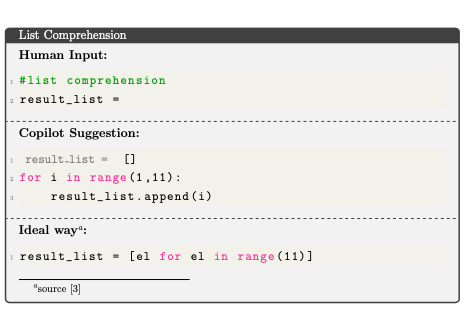
\includegraphics[width=\linewidth]{Figures/idioms_1.png}
    \caption{List Comprehension Idiom and Copilot Suggestion}
    \label{fig:idioms_1}
\end{figure}

The results show that Copilot did not suggest the optimal way as its first suggestion in the majority of the idioms we tested. This shows that current \cct{} like Copilot cannot suggest the idiomatic way in every suggestion even though they are the top most frequently used python idioms in public repositories on GitHub~\cite{Alexandru2018}. 

Copilot being closed source we cannot investigate the potential reasons behind this behavior. However, one plausible explanation for this behavior is that idiomatic ways may not be as frequent as non-idiomatic ways in Copilot's training data of public repositories on GitHub, making the non-idiomatic way rank higher than the idiomatic way.

\cct{} like Copilot should learn to detect idiomatic ways in public repositories and rank them higher than the most frequently used way in public repositories, so that the first suggestion would be the idiomatic way rather than the non-idiomatic way, which is the desirable way for \cct{} like Copilot. For the scope of this thesis, we leave resolving this problem as future work.

% \begin{tcolorbox}[title=List Comprehension,boxsep=.25mm]
%     %https://tex.stackexchange.com/questions/337909/tcolorbox-tcbline-style
% \textbf{Human Input:}
% \begin{lstlisting}[language={Python}]
% #list comprehension
% result_list = 
% \end{lstlisting}
% \tcbline
% \textbf{Copilot Suggestion:}
% \begin{lstlisting}[language=Python,escapechar=\%]
% % \noindent\textcolor{gray}{result\_list  =} % []
% for i in range(1,11):
%     result_list.append(i)
% \end{lstlisting}
% \tcbline
% \textbf{Idiomatic way\footnote{source \cite{Alexandru2018}}:}
% \begin{lstlisting}[language=Python]
% result_list = [el for el in range(11)]
% \end{lstlisting}
% \end{tcolorbox}

%%%%%% TODO: remember to update the screenshot if the source citation is different from the citation in the text %%%%%%

All the Idioms shown in Table~\ref{tab:all_idioms} can be found in the \repl{} including the code used as input (i.e., human input), the top suggestion by Copilot and the idiomatic way suggested in Alexandru et al.~\cite{Alexandru2018}.

\subsection{Code Smells}
\label{smells}
Using the methodology described in section~\ref{smells:methodology}, we sampled 10 best practices in javascript from AirBNB javascript coding style guide~\cite{airbnb_code} and compared Copilot syggestions when prompted with a input method(shown in section~\ref{smells:input}) and evaluated using methodology shown in section~\ref{smells:evaluation}. 

Copilot suggested the best practice from the coding guide for only one out of the ten coding standards we tested, i.e, 1 out of 10 instances Copilot had the recommended way as its top suggestion. Moreover, only 2 out of remaining 9 standards had the best practice in Copilot top 10 suggestions currently viewable. Copilot did not have the best practice in any of its top 10 suggestions for 7 standards out of 10 coding standards we tested.

% Copilot performed significantly worse than the Pythonic Idioms we showed in Section~\ref{secidioms}, As Copilot is closed source, we cannot find the reason behind this but one could argue that lack of data for JavaScript compared to python could be a reason for this behaviour. 

Table~\ref{tab:all_bp} shows the complete list of all the coding standards we tested on Copilot sampled from the AirBNB Coding Style guide~\cite{airbnb_code} and the ranking of the best practice in Copilot suggestions (if it exists).

\begin{table}[ht]
    \centering
    \begin{tabular}{|L|c|}
    \hline
         \textbf{Best Practice  Title} & \textbf{Copilot Suggestion Matched?} \\
         & (out of 10 suggestions) \\
         \hline
         Usage of Object method shorthand & No \\
         \hline
         Array Creating Constructor & 6\textsuperscript{th} \\
         \hline
         Copying Array Contents  & No \\
         \hline
         Logging a Function &  No \\
         \hline
         Exporting a Function & No \\
         \hline
         Sum of Numbers & 9\textsuperscript{th} \\
         \hline
         Accessing Properties & 1\textsuperscript{th} \\
         \hline
         Switch case usage & No \\
         \hline
         Return value from Function with a condition check & No \\
         \hline
         Converting Array-like object to an Array  & No \\
         \hline
    \end{tabular}
    \caption{List of all JavaScript Best Practices tested on Copilot.}
    \label{tab:all_bp}
\end{table}

Figure~\ref{fig:bp_1} shows the Best Practice for Copying Array Contents, showing user input (i.e., Human Input), the top suggestion by Copilot and the recommended way suggested by AirBNB JavaScript coding style guide~\cite{airbnb_code}.

\begin{figure}[hbt!]
    \centering
    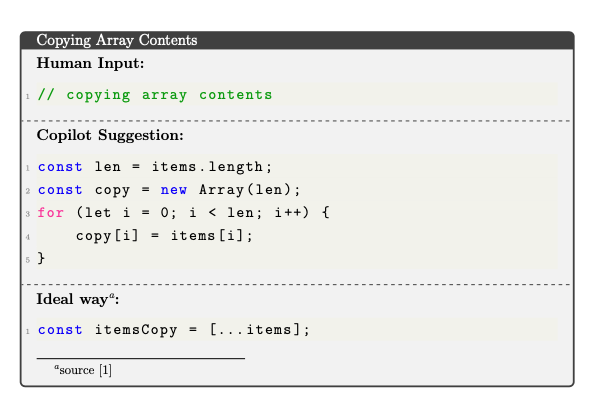
\includegraphics[width=\linewidth]{Figures/bp_1.png}
    \caption{Best Practice for Copying Array Contents and Copilot Suggestion.}
    \label{fig:bp_1}
\end{figure}

The results show that Copilot performed worse than the language idioms~(shown in chapter~\ref{chapter:idioms}). Copilot did not suggest the best practice as its first suggestion for 7 out of 10 coding standards we tested. This shows that current AI-supported
code completion tools like Copilot cannot suggest coding standards in its suggestions even though the coding standards are the sampled from widely accepted coding style guide.

All the Best Practices shown in Table~\ref{tab:all_bp} can be found in the \repl{} including the code used as input (i.e., human input), the top suggestion by Copilot and the best practice from AirBNB JavaScript coding style guide~\cite{airbnb_code}.

There could be many reasons for this performance like the public repositories do not always follow coding standards, Copilot cannot detect coding style from repositories that have contribution guides including the coding standards followed in the project. 
Copilot being closed source we cannot investigate the potential reasons behind this behavior and recommend ways to fix this issue improving the performance of Copilot.

We did not test Copilot for suggesting project specific coding styles because Copilot does not have the feature to customise its suggestions based on preferences~\cite{Copilot-web}.
However, \cct{} like Copilot should follow coding style guides and adapt their code suggestions to match the coding style used in the project. 
For example, if a user is working on a project where one of the coding style guideline says to leave a blank line after blocks and before the next statement~\cite{airbnb_code}. As a productivity tool, the ideal behaviour for \cct{} like Copilot is to detect the coding style guideline from existing code in the project and always suggest code that follows the guideline. 

% \begin{tcolorbox}[title=Copying Array Contents,boxsep=.15mm]
%     %https://tex.stackexchange.com/questions/337909/tcolorbox-tcbline-style
% \textbf{Human Input:}
% \begin{lstlisting}[language=JavaScript]
% // copying array contents
% \end{lstlisting}
% \tcbline
% \textbf{Copilot Suggestion:}
% \begin{lstlisting}[language=JavaScript]
% const len = items.length;
% const copy = new Array(len);
% for (let i = 0; i < len; i++) {
% 	  copy[i] = items[i];
% }
% \end{lstlisting}
% \tcbline
% \textbf{Ideal way\footnote{source \cite{airbnb_code}}:}
% \begin{lstlisting}[language=JavaScript]
% const itemsCopy = [...items];
% \end{lstlisting}
% \end{tcolorbox}

%%%%%% TODO: remember to update the screenshot if the source citation is different from the citation in the text %%%%%%


\subsection{Summary of Findings}
In an attempt to find the boundaries of \cct{} like Copilot, we analyzed Copilot code suggestions for Pythonic idioms and JavaScript best practices. 
We identified that Copilot did not suggest the idiomatic way as its top suggestion for 23 out of 25 coding scenarios in Python. 
Furthermore, we identified that Copilot did not suggest the recommended best practice for 22 out of 25 coding scenarios in JavaScript.

Although Copilot is very good at solving well-specified programming contest style problems~\cite{empirical_eval}, our experiments show that it does not do well in following idioms and recommending best practices in its code suggestions.
Additionally, \cct{} like Copilot being a productivity tool, should be able to suggest idiomatic approaches and recommended best practices in its code suggestions to be helpful for the user.
Studies like ours might help use this delineation to understand what might help turn \cct{} such as Copilot into full-fledged \AISE{} tools.
\section{Chapter Summary}
In summary, we start this chapter by showing the methodology used in addressing textbf{RQ-1} (What are the current boundaries of \cct{}?). 
We first introduced Pythonic idioms and best practices in JavaScript.
We then present our sampling approach for sampling 25 coding scenarios to analyze Copilot code suggestions.
Furthermore, we discussed the input given to Copilot to trigger a code suggestion 
and how the input was restricted to deriving the desired way from the input.
Finally, we described our evaluation approach for Copilot code suggestions.

We sampled 25 Pythonic idioms from Alexandru et al.~\cite{Alexandru2018}, and Farook et al.~\cite{idioms}.
We identified that Copilot did not suggest the idiomatic way as its top suggestion for 23 out of 25 coding scenarios in Python, which addressed \textbf{RQ-1.1} (How do \cct{} manage programming idioms?).
Furthermore, we sampled 25 best practices in JavaScript from the AirBNB JavaScript coding style guide~\cite{airbnb_code}. We identified that Copilot did not suggest the recommended best practice for 22 out of 25 coding scenarios in JavaScript, which addressed \textbf{RQ-1.2} (How do \cct{} manage to manage to suggest non-smelly code?).


% we showed that Copilot struggles to detect and most common idiomatic ways present in public repositories of GitHub and rank them higher than the non-idiomatic ways. The ideal behavior of \cct{} like Copilot in solving this problem is detecting common patterns present in code and rank them higher as the idiomatic ways for a task.
% In the next chapter (chapter~\ref{smells}), we look into how this ideal behavior can cause problems in the case of code smells, where common bad practices present in public repositories of GitHub can make \cct{} like Copilot introduce bad coding practices in its suggestions.

% % \section{Chapter Summary}
% In summary, we start this chapter by showing the methodology used in addressing \textbf{RQ-1.2} (How do \cct{} manage to suggest non-smelly code?). We first introduced the study setup with the input to Copilot and how it was restricted to deriving the best practice from the input and how the suggestions from Copilot were evaluated. We sampled best practices from AirBNB JavaScript coding style guide~\cite{airbnb_code}, and then compared it against Copilot suggestions. Based on results shown in Table~\ref{tab:all_bp}, Copilot struggles to suggest the best practices from widely used coding standards in its suggestions. 

In this chapter, we showed that Copilot struggles to detect and follow coding style guides present in public repositories of GitHub and always suggests code that follows those coding style guides. We also observed that Copilot struggles to detect and most common idiomatic ways present in public repositories of GitHub and rank them higher than the non-idiomatic ways. 
Identifying this delineation could help in urn AI-supported code completion tools such as Copilot into full-fledged AI-supported software engineering tools.
In the next chapter (chapter~\ref{chapter:framework}), we illustrate our taxonomy inspired by autonomous driving levels on the software abstraction hierarchy in \AISE{} and delineate where \cct{} like Copilot currently stands in the taxonomy. 
	\startchapter{Framework}
\label{chapter:framework}

\section{Introduction}
Copilot works best in creating boilerplate and repetitive code patterns~\cite{Copilot-web}.
However, the code suggested by \cct{} like Copilot are found to have simple coding mistakes and security vulnerabilities. Several classes of errors have been discovered, which follow from the presence of these same errors in training data of Copilot~(shown in section~\ref{challenges}).
In Chapter~\ref{chapter:methodology}, we identified that Copilot does not perform well in detecting and suggesting Pythonic idioms and best practices in JavaScript.
The scope of capability and the quality of code suggestions made by \cct{} like Copilot is uncertain. 

In this chapter, we try to create a metric for answering \textbf{RQ-1} (What are the current boundaries of code completion tools) with a taxonomy of six software abstraction levels to help access the current capabilities of \cct{} such as Copilot. 
We explain each software abstraction level in the taxonomy and the capabilities required by \cct{} to satisfy the software abstraction level. 
We try to delineate where current \cct{} such as Copilot, are best able to perform and where more complex software engineering tasks overwhelm them using a software abstraction hierarchy where ``basic programming functionality'' such as code compilation and syntax checking is the lowest abstraction
level, while software architecture analysis and design are at the highest abstraction
level
Additionally, we use a sorting routine as an example scenario to show how a \cct{} code suggestion looks like in every level of abstraction in our taxonomy.

Finally, we try to address \textbf{RQ-2} (Given the current boundary, how far is it from suggesting design decisions?) with a discussion on the level of complexities and challenges involved in creating \cct{} that can satisfy design level compared to \cct{} satisfying code smells level in our taxonomy.

\subsection{Motivation}
To center our analysis on creating a software abstraction hierarchy to create a metric for answering \textbf{RQ-1} (What are the current boundaries of code completion tools), 
we leverage an analogous concept in the more developed (but still nascent) field of autonomous driving. 
Koopman has adapted the SAE Autonomous Driving safety levels~\cite{sae} to seven levels of autonomous vehicle safety hierarchy of needs shown in figure~\ref{fig:koopman_pyramid}. 

\begin{figure}[hbt!]
    \centering
    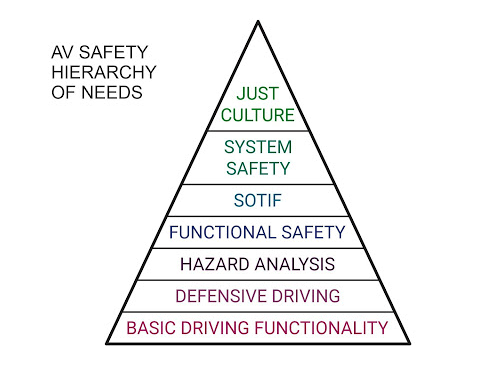
\includegraphics[width=\linewidth]{Figures/koopman_pyramid.png}
    \caption{Koopman's Autonomous Vehicle Safety Hierarchy of Needs~\cite{koopman}. SOTIF = safety of the intended function.}
    \label{fig:koopman_pyramid}
\end{figure}

The pyramid concept is derived from that of Maslow~\cite{Maslow1943}, such that addressing aspects on the top of the pyramid requires the satisfaction of aspects below. 
For example, before thinking about system safety (such as what to do in morally ambiguous scenarios), the vehicle must first be able to navigate its environment reliably (``Basic Driving Functionality'').

We think that a similar hierarchy exists in \AISE{}. Before worrying about software architecture issues, that is, satisfying system quality attributes such as performance and following idiomatic approaches, \AISE{} tools need to exhibit ``basic programming functionality''. This basic functionality is where most research effort is concentrated, such as program synthesis, \cct{}, and automated bug repair.

\section{Taxonomy}
\label{taxonomy}
Our taxonomy is a software abstraction hierarchy where ``basic programming functionality'' such as code compilation and syntax checking is the lowest abstraction level,
Software architecture analysis and design are at the highest abstraction level.
As we ascend the levels, just as with Koopman's pyramid in figure \ref{fig:koopman_pyramid}, 
software challenges rely more on human input and become more difficult to automate (e.g., crafting design rules vs. following syntax rules).

Figure~\ref{fig:taxonomy} shows the taxonomy of autonomy levels for \cct{}. The more abstract top levels depend on the resolution of the lower ones. As we move up the hierarchy, we require more human oversight of the AI; as we move down the hierarchy, rules for detecting problems are easier to formulate. Green levels are areas where \cct{} like Copilot works reasonably well, while red levels are challenging for Copilot based on tests shown in Chapter~\ref{chapter:methodology}.

\begin{figure}[hbt!]
    \centering
    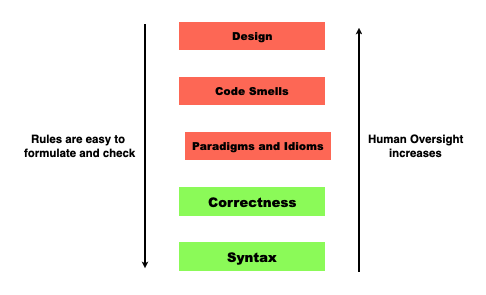
\includegraphics[width=\linewidth]{Figures/taxonomy.png}
    \caption{Hierarchy of software abstractions. Copilot cleared all green levels and struggled in red levels}
    \label{fig:taxonomy}
\end{figure}

Based on our tests with Copilot shown in chapter~\ref{chapter:methodology}, Copilot was able to generate syntactically correct code that solves the given programming task in the coding scenario~(shown in ~\repl{}).
This functionality covers the syntax and the correctness level in our software abstraction hierarchy.
As a result, Copilot stands at the correctness level of our taxonomy. 

The challenges further up the hierarchy are nonetheless more important for software quality attributes (QA)~\cite{Ernst2017} and for a well-engineered software system.
For example, an automated solution suggested by \cct{} to the top level of the taxonomy would be able to follow heuristics to engineer a well-designed software system, which would be easy to modify and scale to sudden changes in use.
\subsection{Syntax}
\label{syntax}
The syntax level is the lowest abstraction level in our taxonomy. This level includes the most basic programming functionality like syntax and code compilations. This level does not require the \cct{} suggested code to successfully perform the task but to suggest code without any obvious errors like syntax errors.

For example, consider a programming task of performing a sorting operation on a list of numbers. 
To satisfy this level of abstraction, \cct{} should suggest code that is syntactically correct without any compilation errors and the code is not required to perform the sorting operation correctly. 
Figure~\ref{fig:syntax} shows the sorting example and Python syntax suggestions from \cct{} at this abstraction level.

\begin{figure}[hbt!]
    \centering
    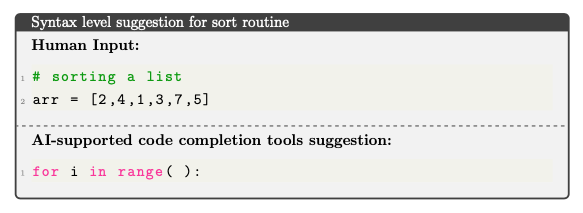
\includegraphics[width=\linewidth]{Figures/syntax.png}
    \caption{code suggestion of \cct{} at syntax level}
    \label{fig:syntax}
\end{figure}

The goal of this software abstraction level in our taxonomy is for a \cct{} to be able to suggest code without any syntactical errors.
The capabilities required by \cct{} to satisfy this level of abstraction are as follows:

\begin{enumerate}
    \item Suggested code should be syntactically correct.
    \item Suggested code should not produce any errors in code compilation.
\end{enumerate}

% \begin{tcolorbox}[title=Syntax level suggestion for sort routine,boxsep=.15mm]
%     %https://tex.stackexchange.com/questions/337909/tcolorbox-tcbline-style
% \textbf{Human Input:}
% \begin{lstlisting}[language={Python}]
% # sorting a list
% arr = [2,4,1,3,7,5]
% \end{lstlisting}
% \tcbline
% \textbf{\cct{} suggestion:}
% \begin{lstlisting}[language={Python}]
% for i in range( ):
% \end{lstlisting}
% \end{tcolorbox}
\subsection{Correctness}
\label{correctness}
Correctness is the second level of software abstraction in our taxonomy. 
\cct{} at this level should be capable of suggesting code that is not only syntactically correct but also solves the programming task. 
This level does not require \cct{} to suggest the best possible coding solution for the programming task but to be able to suggest a decent solution to the programming task which may or may not resolve all the edge cases of the given programming task.

For example, consider the programming task of performing a sorting operation on a list of numbers. To satisfy this level of abstraction, \cct{} should suggest a syntactically correct list sorting code, which is not required to be the most efficient way of sorting a list.
Figure~\ref{fig:correctness} shows the list sorting example and the Python code suggestion from \cct{} at this abstraction level, which performs the sorting operation.

\begin{figure}[hbt!]
    \centering
\begin{tcolorbox}[title=Correctness level suggestion for sort routine,boxsep=.15mm]
    %https://tex.stackexchange.com/questions/337909/tcolorbox-tcbline-style
\textbf{Human Input:}
\begin{lstlisting}[language={Python}]
# sorting a list
arr = [2,4,1,3,7,5]
\end{lstlisting}
\tcbline
\textbf{\cct{} suggestion:}
\begin{lstlisting}[language={Python}]
n = len(arr)
for i in range(n):
    for j in range(n-1):
        if arr[j] > arr[j+1]:
            temp = arr[j]
            arr[j] = arr[j+1]
            arr[j+1] = temp
print(arr)
\end{lstlisting}
\end{tcolorbox}
    \caption{Code suggestion of \cct{} at correctness level.}
    \label{fig:correctness}
\end{figure}

The goal of this software abstraction level in our taxonomy is for a \cct{} to be able to suggest a solution instead of the best one.
The capabilities required by \cct{} to satisfy this level of abstraction are as follows:

\begin{enumerate}
    \item Suggest a solution for a given programming task that may not be the optimal solution for that programming task.
    \item The solution suggested is not required to cover all the edge cases for that programming task.
    \item Satisfy requirements of all the levels below correctness in our taxonomy.
\end{enumerate}


\subsection{Paradigms and Idioms}
Paradigms and idioms are our taxonomy's third level of software abstraction. 
This level requires the code suggested by \cct{} to satisfy all the previous levels of abstractions and use common paradigms and language idioms in its code suggestions. 
These include common practices of solving a programming task. 

Returning to our running example of performing a sorting operation on a list of numbers. 
To satisfy this level of abstraction, \cct{} should suggest a syntactically correct list sorting code, using idiomatic ways in its code suggestions, like the Pythonic way of swapping items in a list~(line 5 in figure~\ref{fig:idioms}), As opposed to suggesting non-idiomatic approaches like creating another temporary variable to swap items in a list shown in correctness level~(figure~\ref{fig:correctness}).

Figure~\ref{fig:idioms} shows the sorting example and the Python code suggestions from \cct{} at this abstraction level.

\begin{figure}[hbt!]
    \centering
\begin{tcolorbox}[title=Idioms level suggestion for sort routine,boxsep=.15mm]
    %https://tex.stackexchange.com/questions/337909/tcolorbox-tcbline-style
\textbf{Human Input:}
\begin{lstlisting}[language={Python}]
# sorting a list
arr = [2,4,1,3,7,5]
\end{lstlisting}
\tcbline
\textbf{\cct{} suggestion:}
\begin{lstlisting}[language={Python}]
n = len(arr)
for i in range(n):
	for j in range(n-1):
		if arr[j] > arr[j+1]:
			arr[j], arr[j+1] = arr[j+1], arr[j]
print(arr)
\end{lstlisting}
\end{tcolorbox}
    \caption{Code suggestion of \cct{} at paradigms and idioms level.}
    \label{fig:idioms}
\end{figure}

The goal of this software abstraction level in the taxonomy is for \cct{} to detect and use commonly known idiomatic approaches and paradigms that occur in public code in its suggestions for suggesting code to solve a programming task.

The capabilities required by \cct{} to satisfy paradigms and idioms level of software abstraction are as follows:
\begin{enumerate}
    \item Identify common patterns like paradigms and language idioms in public code repositories~(training data).
    \item Use paradigms and language idioms in suggesting solutions for a programming task.
    \item Satisfy requirements of all the levels below paradigms and idioms in our taxonomy.
\end{enumerate}


\section{Design Smells}
Currently, Copilot does not support multi-file input, So it is not possible to evaluate its design suggestions, as software development process may include multiple folders with a file structure. 
Making Code completion tools adapt their suggestions to context specific issues such as variable naming conventions and formatting would be challenging as the existing guidelines are not standard in this space and mostly depend on context, The training dataset for AI driven development should also include rules such as idioms, best practices before tackling design level problems.
% Design smells or arch smells (Tushar Sharma)
\subsection{Design level}
Software design is the highest level of abstraction in our taxonomy. The goal of this level is to make \cct{} support the user in every software development process and suggest improvements.
To simplify the taxonomy of overall design processes in software development, we divided it into two subcategories: Module level design and System level design. 
\cct{} at the Module level design requires more user involvement in making design choices at the file level. Whereas, in system level design, \cct{} are more autonomous and require minimal input from the user in making design choices.

\subsubsection{Module level design}
\label{low_design}
Module level design is the first half of our taxonomy's design level of software abstraction.
This level requires the suggested code to be free of all known vulnerabilities and include test cases and continuous integration methods when applicable.
Code suggestions should also cover all the functional requirements of a given programming task.

\cct{} at this level should be able to pick and suggest the best applicable algorithm for a given coding scenario and be capable of following user-specified coding style guidelines.
For example, consider the task of sorting operation on a list of numbers. To satisfy this level of abstraction, \cct{} should suggest a syntactically correct list sorting code, using an algorithm that gives the best performance for that particular input scenario, like suggesting a quick sort algorithm~(avg time complexity = nlogn) instead of bubble sort algorithm~(avg time complexity = n\textsuperscript{2}).

The goal of this level in the taxonomy is for a \cct{} to be able to suggest appropriate design choices at the file level, considering the input from the user, like coding style guidelines, and help the user make design choices that satisfy all the functional requirements of the given programming task.

The capabilities required by a \cct{} to satisfy this level of abstraction are as follows
\begin{enumerate}
    \item Picking and suggesting the best applicable algorithm for a given scenario.
    \item Identify file level concerns in code files.
    \item Code suggestions should be free from all recognized vulnerabilities and warn the user if a vulnerability is found.
    \item Code suggestions should cover all the functional requirements of the given programming task.
    \item \cct{} should be able to suggest code with appropriate tests and Continuous Integration~(CI) when applicable.
    \item Code suggestions should follow user-specified coding style guidelines.
    \item Satisfy requirements of all previous levels of abstractions.
\end{enumerate}

% \begin{tcolorbox}[title=Code smells level suggestion for sort routine,boxsep=.15mm]
%     %https://tex.stackexchange.com/questions/337909/tcolorbox-tcbline-style
% \textbf{Human Input:}
% \begin{lstlisting}[language={Python}]
% # sorting a list
% arr = [2,4,1,3,7,5]
% \end{lstlisting}
% \tcbline
% \textbf{\cct{} suggestion:}
% \begin{lstlisting}[language={Python}, morekeywords={False, True}]
% swapped = False
% for i in range(len(arr)-1, 0, -1):
% 	for j in range(n):
% 		if arr[j] > arr[j+1]:
% 		    swapped = True
% 			arr[j], arr[j+1] = arr[j+1], arr[j]
% 	if not swapped:
% 	    break
% print(arr)
% \end{lstlisting}
% \end{tcolorbox}
\subsubsection{System level design}
\label{high_design}
System level design is the second half of the design level in our taxonomy. This level is the highest abstraction level with the highest human oversight and the most complex to define rules.
\cct{} at this level can suggest design decisions at the project level, like suggesting design patterns and architectural tactics with minimal input from the user.

This level requires the suggested code to suggest rational design practices in its code suggestions for a problem and satisfy all the previous levels of abstractions. Design practices depend on many factors like requirements and technical debt. \cct{} should be capable of considering all the relevant factors before suggesting a design practice and providing the reasoning for each choice to the user.

The main goal of this level in the taxonomy is for a \cct{} to help the user in every part of the software development process with minimal input from the user.

The capabilities required by a \cct{} to satisfy this level of abstraction are as follows
\begin{enumerate}
    \item Identify system level concerns in code files.
    \item Suggest design patterns and architectural tactics when prompted.
    \item Code suggestions should cover all the project's non-functional requirements.
    \item \cct{} should be able to identify the coding style followed and adapt its code suggestions.
    \item \cct{} should be able to make design decisions based on requirements and inform the user about those decisions.
    \item Satisfy requirements of all previous levels of abstractions.
\end{enumerate}

To make a \cct{} suggest design decisions is a very challenging task. 
Software design is very subjective, and software design concerns are still challenging to comprehend. 
This is because software design is one of the least concrete parts of the software development lifecycle, especially compared to testing, implementation, and deployment~\cite{sedesign}. 
Software design is typically carried out heuristically by drawing on the design team's knowledge, the project context (such as architecturally significant needs), and a constantly evolving set of patterns and styles from the literature. We discuss more on these challenges in Chapter~\ref{chapter:discussion}.
\section{AI-supported Software Development}
\label{cs2design}
We began this thesis by analyzing Copilot code suggestions on Pythonic idioms and best practices in Javascript to understand the current boundaries of \cct{} like Copilot using a software abstraction taxonomy.
In this section, we try to address \textbf{RQ-2} (Given the current boundary, how far is it from suggesting design decisions?) with a discussion on the complex nature of design decisions involving factors ranging from requirement analysis to maintenance, making it difficult for \cct{} like Copilot to detect the information from code files and suggest design decisions to satisfy the top software abstraction level of our taxonomy.
Additionally, we discuss our vision for \cct{} like Copilot to satisfy the design level in our taxonomy and outline the difficulty its underlying Codex LLM approach might run into.
Finally, we discuss how design choices change over time and outline the difficulties of \cct{} like Copilot to keep updating its suggestions and reflect the current design practices~(section~\ref{evolution}).

Software development is a challenging, complex activity: It is common for tasks to be unique and to call for the analysis of ideas from other domains. Solutions must be inventively modified to address the requirements of many stakeholders.
Software design is a crucial component of the software development activity since it determines the various aspects of the system, such as its performance, maintainability, robustness, security, etc.
Design is typically viewed in the context of software engineering as both a process~\cite{design} that a development team engages in and the specifications~\cite{designdef} that the team produces. 
Software design is typically carried out heuristically by pulling from the project context (such as architecturally significant needs), the design team's knowledge, and a constantly evolving set of patterns and styles from the literature. 

Automating this software design process, which is the most abstract element in the software development lifecycle, will be challenging. 
First, sufficient software design knowledge has to be collected to use as training data to create a good \cct{} that can suggest relevant architectural patterns. 
Software design generally occurs in various developer communication channels such as issues, pull requests, code reviews, mailing lists, and chat messages for multiple purposes such as identifying latent design decisions, design challenges, design quality, etc. 
Gathering all this data and generalizing those design decisions in training data to suggest relevant design choices to a user would be the vision for \cct{} to satisfy the design level.

Stack Overflow\footnote{\url{https://stackoverflow.com/}}, the most popular question and answer (Q\&A) forum used by developers for their software development queries~\cite{sotorrent}.
Software developers of all levels of experience conduct debates and deliberations in the form of questions, answers, and comments on Stack Overflow's extensive collection of topics about software development.
Due to these qualities, Stack Overflow is a top choice for software developers looking to crowdsource design discussions and judgments, making it a good source of training data for \cct{} for design choices.

Additionally, \cct{} at the design level should be capable of capturing design and module level concerns. 
These include capturing design patterns~(such as Observer) and architectural tactics~(such as Heartbeat) to improve and personalize suggestions.
The general understanding of a system's design that a software developer has is frequently susceptible to ``evaporation," which causes the developers to gradually lose knowledge of the design over time~\cite{martinse} making the process of gathering design data to train \cct{} a significant challenge.

Organizing software design information is an active research area. Previously, this design knowledge was organized largely manually because the information was heavily context-specific and a lack of large datasets. A study by Gorton et al.~\cite{databases} showed a semi-automatic approach to populate design knowledge from internet sources for a particular (big data) domain, which can be a helpful approach for collecting software design relevant data to train \cct{}.

Over the natural evolution of a software system, small changes accumulate, which can happen for various reasons, such as refactoring~\cite{fabio}, bug fixes~\cite{cotroneo}, implementation of new features, etc.
These changes can be unique. However, they frequently repeat themselves and follow patterns~\cite{changes}. 
Such patterns can provide a wealth of data for studying the history of modifications and their effects~\cite{martinchanges}, modification histories of fault fixes~\cite{daniel}, or the connections between code change patterns and adaptive maintenance~\cite{ijece}.
However, to use this data, \cct{} should be able to identify these complex patterns existing in public code~(training data). Current \cct{} like Copilot struggled to detect much simpler patterns like Pythonic idioms. There is no evidence currently to suggest they can identify even more complex design patterns.

Additionally, current \cct{} like Copilot does not support multi-file input. It is not possible to evaluate its current performance in design suggestions, as the software development process may include multiple folders with a file structure. 
For example, MVC pattern generally includes multiple files acting as Model, View, and Controller. Using the current limitations of input on Copilot, i.e., a code block or a code file, it is not possible for \cct{} to deduce that the project is using the MVC pattern and adapt its suggestion to follow the MVC pattern and not suggest code where Model communicated directly with View. \cct{} must be capable of making suggestions in multiple program units to accommodate these more abstract design patterns.

\cct{} should be able to adapt their suggestions to context-specific issues such as variable naming conventions and formatting. 
This would be challenging as the existing guidelines are not standard in this space and mostly depend on context.

\subsection{Evolution of design over time}
\label{evolution}
Software design is an ever-changing field that evolves along with technology, languages, and frameworks. As a result, either new design patterns are developed, or some existing ones are depreciated.
\cct{} need to update their code suggestions regularly to reflect the changes in design practices. 
This requires regularly updating the training data, and training costs are expensive.

Design patterns are solutions to recurring design issues that aim to improve reuse, code quality, and maintainability.
Design patterns have benefits such as decoupling a request from particular operations~(Chain of Responsibility and Command), making a system independent from software and hardware platforms~(Abstract Factory and Bridge), and independent from algorithmic solutions~(Iterator, Strategy, Visitor), or preventing implementation modifications~(Adapter, Decorator, Visitor). These design patterns are integral to software design and are used regularly in software development.
However, these design patterns evolve. For instance, with React Framework's introduction, many new design patterns were introduced, such as Redux and Flux, which were considered to be an evolution over the pre-existing MVC design pattern.
\cct{} trained before this evolution will not have any data of the new design patterns such as Redux and Flux, making them incapable of suggesting those design patterns to the user. 

Similarly, coding practices evolve. 
For example, in JavaScript, callbacks were considered the best practice in the past to achieve concurrency, which was replaced by promises. 
When the user has a goal to achieve asynchronous code, there are two ways to create async code: callbacks and promises. Callback allows us to provide a callback to a function, which is called after completion. With promises, you can attach callbacks to the returned promise object.
One common issue with using the callback approach is that when we have to perform multiple asynchronous operations at a time, we can easily end up with something known as callback hell.
As the name suggests, it is harder to read, manage, and debug. The simplest way to handle asynchronous operations is through promises. In comparison to callbacks, they can easily manage many asynchronous activities and offer better error handling.
This makes \cct{} be updated regularly to reflect new changes in coding practices and design processes of software development. 

Additionally, Bad Practices in using promises for asynchronous JavaScript like not returning promises after creation and forgetting to terminate chains without a catch statement, which are explained in documentation\footnote{\label{docs}\url{https://developer.mozilla.org/en-US/docs/Web/JavaScript/Guide/Using_promises}} and StackOverflow\footnote{\url{https://stackoverflow.com/questions/30362733/handling-errors-in-promise-all/}} are not known to Copilot and suggested code with those common anti-patterns as they could have occurred more frequently in Copilot training data. 
While testing, Copilot suggested code specifically mentioned in the JavaScript documentation as a common bad practice and anti-pattern\footref{docs}.
However, this is beyond the scope of this study and will be part of future work.

In conclusion, Software design is an abstract field of software development, where humans struggle to make correct design decisions using all their previous experience and various sources of information to satisfy the requirements of a system. 
Creating \cct{} to automate the software design process requires gathering relevant training data and regular updates to the training data to reflect the new changes in the evolution of the software development process. Further, the current Copilot approach of token-level suggestions needs to be upgraded to move beyond tokens~(shown in \ref{tokens}) to facilitate multi-file input to help make \cct{} capable of satisfying the design level of our taxonomy.
\section{Chapter Summary}
In summary, we start this chapter by showing the methodology used in addressing \textbf{RQ-1.2} (How do \cct{} manage to suggest non-smelly code?). We first introduced the study setup with the input to Copilot and how it was restricted to deriving the best practice from the input and how the suggestions from Copilot were evaluated. We sampled best practices from AirBNB JavaScript coding style guide~\cite{airbnb_code}, and then compared it against Copilot suggestions. Based on results shown in Table~\ref{tab:all_bp}, Copilot struggles to suggest the best practices from widely used coding standards in its suggestions. 

In this chapter, we showed that Copilot struggles to detect and follow coding style guides  present in public repositories of GitHub and always suggest code that follows those coding style guides. The ideal behavior of \cct{} like Copilot in solving this problem is to detect the coding style guideline from existing code in the project and always suggest code that follows the guideline.

In the next chapter (chapter~\ref{chapter:framework}), we illustrate our taxonomy inspired from autonomous driving levels on the software abstraction hierarchy in \AISE{}, and delineate where \cct{} are currently best able to perform, and where more complex software engineering tasks overwhelm them.
	\startchapter{Discussion, Future Work and Conclusion}
\label{chapter:discussion}

\section{Introduction}
We began this thesis with an analysis of Copilot code suggestions on Pythonic idioms, and Javascript best practices to understand the current boundaries of AI-supported code completion tools like Copilot using a software abstraction taxonomy. 
In this chapter, we first begin by extending this discussion by comparing Copilot performance on Pythonic idioms and JavaScript best practices. In section~\ref{performance}, we discuss the differences in the performance and ranking of Copilot code suggestions on Pythonic idoms and JavaScript best practices. We also discuss how Copilot was able to suggest idiomatic code for some coding scenarios.

Furthermore, having established the software abstraction hierarchy to help assess the capabilities of \cct{}, 
in section~\ref{recite}, we discuss what it means to recite code from training data of \cct{} like Copilot.
Additionally, we discuss how code recitation is an ideal behavior for \cct{} like Copilot to suggest idiomatic code but not for code smells.

In this second part of this thesis, we discussed our taxonomy of software abstractions and the challenges involved in creating \cct{} that are capable of satisfying the design level of our taxonomy. In section~\ref{implications}, we report on some implications for researchers and practitioners.
Finally, in section~\ref{limitations}, we report on the threats to the validity of the research presented in this thesis.

% We conclude this chapter by discussing how this study could be extended further, some implications for researchers and practitioners, and some future works that our study enables~(section~\ref{future}).

\section{Copilot code suggestions}
\label{performance}
% in the discussion, speculate on why there is variance. When I say “speculate” I mean offer some reasoning that follows a logical process, based on some evidence. WHy is “accessing properties” #1 but “array callback” is lower? What are the commonalities here? 
Copilot code suggestions for our coding scenarios in Pythonic idioms and JavaScript best practices~(shown in Chapter~\ref{chapter:methodology}) has three possible outcomes: Copilot suggesting the recommended approach as its top suggestion~(ideal behavior), Copilot having the recommended approach in its top 10 code suggestions but not the top suggestion~(less ideal) and Copilot does not have the recommended approach in any of its suggestions~(worst case).

Copilot recommending the idiomatic approach as its \emph{top suggestion} is the ideal behavior for all \cct{}.
This may require the recommended approach to be the most popular method to solve the programming task. For example, Copilot successfully suggested the idiomatic approach as its top suggestion for idioms 7~(set comprehension) and 10~(if condition check value). 
Both those programming tasks do not have more than 2 popular methods of solving the problem. Similarly, for code smells, Copilot successfully suggested the JavaScript best practice as its top suggestion for best practices 7~(accessing properties), 15~(converting array-like object to array), and 23~(check boolean value). These programming tasks also have the best practice approach as the most common approach used. 
To make \cct{} like Copilot suggest recommended approach as the top code suggestion, the approach must be the most common way of solving the given programming task. 

Copilot recommending the idiomatic approach in its \emph{top 10 suggestions} is not the ideal behavior but better than not having the idiomatic approach in its suggestions at all. 
Copilot had 8 idiomatic approaches and 5 best practices in its top 10 suggestions. This case is a result of \cct{} having the recommended approach in its training data, but the ranking metrics such as the popularity of the approach made the idiomatic approach rank below the non-idiomatic approach. 
To resolve this case, \cct{} like Copilot should update their ranking approach to have multiple metrics such as repository popularity or acceptance of the approach in online forums such as StackOverflow to make the idiomatic approach rank higher than the non-idiomatic approaches.

When the idiomatic approach is \emph{not in any of its top 10 suggestions}, \cct{} like Copilot does not have the recommended approach in its training data, making it unaware of the approach or the recommended approach is very rare that it didn't even make it to top 10 suggestions, this is the worst case of all three outcomes of our coding scenarios with Copilot. 
This also suggests that people do not use the recommended approach in their code, and efforts should be made to improve awareness of such recommended approaches to solve those common programming tasks.
\section{Copilot Code Recitation}
\label{recite}
% not here but in the discussion the thesis should discuss what it means to “recite” an idiom. Why or why not does Copilot not recommend a particular idiom? Readers will not understand the technical reasons - explain it.

\cct{} like Copilot are trained on billions of lines of code. The code suggestions Copilot makes to a user are adapted to the specific coding scenario, but the processing behind each code suggestion is ultimately taken from training~(public) code.
A recent study conducted by Bender et al.~\cite{stochastic_parrots} showed that LLMs like GPT-3~\cite{Gpt3} and Codex~\cite{copilot} could recite code suggestions identical to the code present in training data, which in turn can cause issues like license infringements~\cite{code_clone}.

Traditional N-gram LMs like SLANG~\cite{slang} and CACHECA~\cite{cacheca}~(shown in section~\ref{ngrams}) can only model relatively local dependencies, predicting each word given the preceding sequence of N words (usually 5 or fewer).
However, more advanced models like the Transformer LMs used in Codex~\cite{copilot} capture much larger windows and can produce code that is seemingly not only fluent but also coherent even over large code blocks. We were able to generate a whole 980 lines of a code file using Copilot with an input of the first 15 lines of that file\footnote{all experiments are documented in \repl{}}.  

This code recitation behavior of LLMs like Codex~\cite{copilot} can help with satisfying paradigms and idioms level of our taxonomy.
Idioms are the most accepted approaches in public~(training) data. 
The ideal behavior of \cct{} like Copilot is to recognize these idiomatic approaches to solve a programming task from training data and use them in code suggestions.

Similarly, Copilot can also recite common code smells in public~(training) data. \cct{} like Copilot needs to recognize the difference between an idiomatic approach and a code smell in training data. 
Metrics like code repository popularity and StackOverflow upvotes on the code can help \cct{} like Copilot to distinguish between idiomatic approaches and code smells. 
\section{Implications}
\label{implications}
% Practical implications can be separated into two categories, pre-training and at suggestion time. 
This research helps guide future \cct{} to support software development. 
Good \cct{} has many potential uses, from recommending expanded code completions to optimizing code blocks. Automating code production could increase the productivity of current programmers. 

Future code generation models may enable developers to work at a higher degree of abstraction that hides specifics, similar to how contemporary software engineers no longer frequently write in assembly.
Good \cct{} may improve accessibility to programming or aid in training new programmers. Models could make suggestions for different, more effective, or idiomatic methods to implement programs, enabling one to develop their coding style.

\subsection{Implications for practice}
For \emph{pre-training the LLM} (e.g., Codex), \AISE{} tools will need higher-quality training data. This might be addressed by carefully engineering training examples and filtering out known flaws, code smells, and bad practices. Careful data curation seems to be part of the approach already~\cite{alphacode}. However, there is little clarity on how this process happens and how to evaluate suggestions, particularly for non-experts. One approach is to add more verified sources like well-known books and code documentation pages to follow the best practices. 
Pre-training might rank repositories for training input according to code quality (e.g., only repositories with acceptable coding standards).
%The goal here is to make good practices more frequent than the bad ones to make Copilot suggest good code as its top suggestion.

For \emph{code completion time}, \AISE{} tools could collaborate with, or be used in conjunction with, existing tools for code smells like SonarQube\footnote{https://www.sonarqube.org} or other code review bots to potentially improve the quality of suggestions. Since developers expect to wait for a code suggestion, the results could be filtered for quality. 
Amazon's code completion tool `CodeWhisperer' comes with a `run security scan' option, which performs a security scan on the project or file that is currently active in VS Code~\cite{amazon}.
Active learning approaches which learn a user's context (e.g., the company coding style) would also improve suggestion acceptability. %Many of these insights can be taken from existing knowledge in the information retrieval domain. 

% As code completion tools are used for productivity, they should improve the ranking system to make best solutions appear as top suggestion (it would take more time to go through all suggestions)
% Recommendations to improve \AIDE{}:
% \begin{enumerate}
%     \item add more verified sources like books and documentations to training data.
%     \item perform code smell detection and vulnerability checks before every suggestion and rank them accordingly.
%     \item ranking suggestions based on repository (source of suggestion) popularity.
% \end{enumerate}


\subsection{Implications for researchers}
With a wide range of applications, including programming accessibility, developer tools, and computer science education, effective code generation models have the potential to have a positive, revolutionary effect on society. 
However, like most technologies, these models may enable applications with societal drawbacks that we need to watch out for, and the desire to make a positive difference does not, in and of itself, serve as a defense against harm.
One challenge researchers should consider is that as capabilities improve, it may become increasingly difficult to guard against “automation bias.”

\subsubsection{Moving Beyond Tokens}
\label{tokens}
Another research challenge is to move beyond token-level suggestions and work at the code block or file level (e.g., a method or module). 
Increasing the model input size to span multiple files and folders would improve suggestions. For example, when there are multiple files implementing the MVC pattern, Copilot should never suggest code where \textsf{Model} communicates directly with \textsf{View}. 
\AISE{} tools will need to make suggestions in multiple program units to accommodate these more abstract design concerns.

One suggestion is to use recent ML advances in helping language models `reason', such as the chain of thought process by Wang et al.~\cite{chain_of_thought}. 
Chain-of-thought shows the model and example of reasoning, allowing the model to reproduce the reasoning pattern on a different input.
Such reasoning is common for design questions. 
Shokri~\cite{shokri21} explored this with framework sketches.

For example, using architectural scenarios helps (humans) reason about which tactic is most suitable for the scenario~\cite{kazman98}. This is a version of the chain of thought for designing systems. 
However, we have an imperfect understanding of the strategies that drive human design approaches for software~\cite{Arab2022}. 
\section{Explainability}
\label{explain}
Copilot is closed source, and it is currently not possible to determine the source or the reason behind each suggestion, making it difficult to detect any problems (access is only via an API). 
However, engineering software systems are laden with ethical challenges, and understanding why a suggestion was made, particularly for architectural questions such as system fairness, is essential. 
Probes, as introduced in \cite{karmakar21}, might expand technical insight into the models.

Another challenge is understanding the basis for the ranking metric for different suggestions made by Copilot. 
This metric has not been made public. 
Thus, we cannot determine why Copilot ranks one approach (e.g., non-idiomatic) over the idiomatic (preferred) approach. However, large language model code suggestions are based on its training data~\cite{training_extraction}, so one explanation is that the non-idiomatic approach is more frequent in the training data~\cite{stochastic_parrots}. 
Better characterization of the rankings would allow users to better understand the motivation. 
\section{Control}
\label{control}
Being generative models, tools like Copilot are extremely sensitive to input with stability challenges and to make them autonomous raises control concerns.
For example, if a human asks for a N\textsuperscript{2} sorting algorithm, should Copilot recommend one, or the NlogN alternative? 
Ideally, tools should warn users if prompted to suggest sub-optimal code. 
\AISE{} should learn to differentiate between optimal and sub-optimal code. 
One direction to look at is following commit histories of files, as they are the possible places to find bug fixes and performance improvements.

\section{Threats to Validity}
\label{limitations}
Copilot and its underlying OpenAI Codex LLM are not open sources. 
%Accessing them is restricted to API calls, and General users cannot directly examine the model. 
We base our conclusions on API results, which complicate versioning and clarity. There are several threats to the validity of the work presented in this thesis. In this section, we summarize the dangers and also present the steps taken to mitigate them. We use the stable Copilot extension release (version: 1.30.6165) in Visual Studio Code. %The manual effort needed to query Copilot restricts the ability to use large datasets.

\subsection{Internal Validity}
Copilot is sensitive to user inputs, which hurts replicability as a different formulation of the problem might produce a different set of suggestions. 
Because Copilot uses Codex, a generative model, its outputs cannot be precisely duplicated. Copilot can produce various responses for the same request at . Copilot is a closed-source, black-box application that runs on a distant server and is therefore inaccessible to general users~(such as the author of this thesis).
Thus a reasonable concern is that our (human) input is unfair to Copilot, and with some different inputs, the tool might generate the correct idiom. 
For replicability, we archived all examples in our replication package at \repl{}.
%\neil{can we try this? }\rohith{idioms are mostly one-lined, and longer inputs/suggestions could be described as bad practices/design smells}

\subsection{Construct Validity}
The taxonomy of the software abstraction hierarchy presented in this thesis relies on our view of software abstractions.
Other approaches for classifying software abstractions~(such as the user's motivation for initiating \cct{}) might result in different taxonomy.
The hierarchy of software abstractions presented in this thesis relies on our understanding of software abstractions, and the results of Copilot code suggestions on language idioms and code smells. Further, we present our results using Python and JavaScript. It is possible that using some other programming language or \cct{} might have different results.

We intended to show where Copilot cannot consistently generate the preferred answer. We biased our evaluation to highlight this by choosing input that simulates what a less experienced programmer might enter. 
But we argue this is reasonable: for one, these are precisely the developers likely to use Copilot suggestions and unlikely to know the idiomatic usage.
More importantly, a lack of suggestion stability seems to come with its own set of challenges, which are equally important to understand.

\subsection{Bias, Fairness, and Representation}
Code generation models are susceptible to repeating the flaws and biases of their training data, just like natural language models~\cite{Gpt3}. These models can reinforce and maintain societal stereotypes when trained on a variety of corpora of human data, having a disproportionately negative effect on underprivileged communities. 
Additionally, bias may result in outdated APIs or low-quality code that reproduces problems, compromising performance and security. This might result in fewer people using new programming languages or libraries.

Codex has the ability to produce code that incorporates stereotypes regarding gender, ethnicity, emotion, class, name structure, and other traits~\cite{copilot}.
This issue could have serious safety implications, further motivating us to prevent over-reliance, especially in the context of users who might over-rely on Codex or utilise it without properly thinking through project design.

% (to use an analogy, we would expect all self-driving vehicles to make similar choices when confronted with similar circumstances). 
%this gets to the top levels of Koopmann's pyramid.
% Access to Copilot is currently restricted. 
% Working with GitHub's API - not open
%
%OpenAI and open source

\subsection{Ethical Considerations}
\label{ethics}
Packages or programs created by third parties are frequently imported within a code file. Software engineers rely on functions, libraries, and APIs for the majority of what called as ``boilerplate" code rather than constantly recreating the wheel. 
However, there are numerous choices for each task: For machine learning, use PyTorch or TensorFlow; for data visualization, use Matplotlib or Seaborn; etc.

Reliance on import suggestions from \cct{} like Copilot may increase as they get used to using \cct{}. 
Users may employ the model as a decision-making tool or search engine as they get more adept at "prompt engineering" with Codex. 
Instead of searching the Internet for information on "which machine learning package to employ" or "the advantages and disadvantages of PyTorch vs. Tensorflow," a user may now type "\# import machine learning package" and rely on Codex to handle the rest.
Based on trends in its training data, Codex imports substitutable packages at varying rates~\cite{copilot}, which may have various effects. 
Different import rates set by Codex may result in subtle mistakes when a particular import is not advised, increased robustness when an individual's alternative package would have been worse, and/or an increase in the dominance of an already powerful group of people and institutions in the software supply chain.

As a result, certain players may solidify their position in the package market, and Codex may be unaware of any new packages created following the first collection of training data. The model may also recommend deprecated techniques for packages that are already in use. Additional research is required to fully understand the effects of code creation capabilities and effective solutions.

% Despite the fact that many packages are free, developers and companies with popular packages can earn incentives, and free packages can act as covers for paid items. 
% Therefore, the import patterns used by Codex and other code generation models may have significant economic effects on individuals who create and maintain packages, in addition to possible safety or security effects.

\section{Conclusion}
\label{conclusion}

% Furthermore, we provided implications for our study. Additionally, we recommend moving beyond token-level suggestions and using reasoning methods to make \cct{} reach the highest level of software abstraction in our taxonomy~(design level).
% Finally, we discussed the threats to the validity of our research and the steps taken to address those threats. We concluded by presenting the future directions of our study. 

Chapter~\ref{chapter:methodology} has shown the current challenges of \cct{} like security issues and license infringements. 
We also showed that \cct{} like Copilot struggle to use Pythonic idioms and JavaScript best practices in its code suggestions.

Chapter~\ref{chapter:framework} represents a continuation of our previous work in chapter~\ref{chapter:methodology} by introducing a taxonomy of software abstraction hierarchy to delineate the limitations of \cct{} like Copilot. We also show that Copilot stands at correctness level of our taxonomy.
Finally, we discussed how \cct{} like Copilot can reach the highest level of software abstraction in our taxonomy~(design level). 

The possible applications of large LLMs like Codex are numerous. 
For instance, it might ease users' transition to new codebases, reduce the need for context switching for seasoned programmers, let non-programmers submit specifications, have Codex draught implementations, and support research and education.

GitHub's Copilot and related large language model approaches to code completion are promising steps in \AISE{}.
However, Software systems need more than coding effort. 
These systems require complex design and engineering work to build. 
We showed that while the coding syntax and correctness level of software problems is well on their way to useful support from \cct{} like Copilot, the more abstract concerns, such as code smells, language idioms, and design rules, are far from solvable at present.
% The paper explored potential implications and ways to address these higher abstraction concerns. 
Although far off, we believe \AISE{}, where an AI supports designers and developers in more complex software \emph{development} tasks, is possible.
% API-driven development for recommendations 
	\startchapter{Conclusions}
\label{chapter:concl}

% 	\appendix
% 	\startappendix{Appendix}
\label{chapter:appendix}




% The style of bibliography exemplified here is the "plain",
% normally used in science theses. This is shown
% by the entry {plain} below. Substitute the
% appropriate bibliography style. See also the
% PDF file "InformationOnBibliographyStyles" in this
% directory for more choices.

% The Bibliography file is a BibTex file named
% UVicThesis.bib and called below

	\TOCadd{Bibliography}
%	\bibliographystyle{ACM-Reference-Format}
	\bibliographystyle{plainurl}
	\bibliography{UvicThesis}

\end{document}
